% Bay Wheels OD Demand — CS361 Final Report
\documentclass[conference,10pt]{IEEEtran}

\usepackage{amsmath,amssymb}
\usepackage{graphicx}
\usepackage{booktabs}
\usepackage{microtype}
\usepackage{url}
\usepackage[hidelinks]{hyperref}
\usepackage[natbib=true,style=numeric,sorting=none,maxbibnames=3]{biblatex}
\addbibresource{references.bib}

% Keep figures within column width
\setlength{\fboxsep}{0pt}
\graphicspath{{../figures/}}

\begin{document}

\title{Shift Happens: A Gravity Model for\\Bay Wheels Bike-Share Demand with\\
       Elevation and Weather Covariates}

\author{
  \IEEEauthorblockN{Ryan Catullo}
  \IEEEauthorblockA{Department of Management Science \& Engineering\\
    Stanford University\\
    rcatullo@stanford.edu}
}

\maketitle

% ─────────────────────────────────────────────────────────────────────────────
\begin{abstract}
We fit a Poisson gravity model for hourly origin--destination (OD)
bike-share demand across the Bay Area using 4.7 million Bay Wheels trips
and 604 stations. The model decomposes log-demand into station-level
fixed effects, temporal fixed effects (hour, day-of-week, month), and
continuous covariates: haversine inter-station distance, signed elevation
gain, and four area-wide ERA5-Land weather variables.
A spatial--temporal factorisation reduces gradient cost per L-BFGS-B
\cite{Liu1989} step from $O(I^2 T)$ to $O(I^2)+O(T)$, making 1{,}258
parameters tractable. A null (distance-only) model serves as baseline.
The full model reduces out-of-sample Poisson deviance by 0.57\% over
the null; precipitation carries the strongest weather signal
($\hat\gamma = -0.521$, a 40\% trip reduction per mm/hr), while
elevation gain is negligible at Bay Area scale.
\end{abstract}

% ─────────────────────────────────────────────────────────────────────────────
\section{Introduction}

Bike-share systems generate millions of origin--destination trips whose
spatial and temporal patterns reflect deep interactions between built
environment, weather, and rider preference. Reliable short-horizon demand
forecasts enable rebalancing operations; meanwhile, fitted model
coefficients quantify how infrastructure and weather shape ridership.

Prior work estimates ridership at the station level
\cite{Rixey2013,Faghih2014} or aggregates across time
\cite{Gebhart2014}, but rarely fits a full hourly OD matrix.
Fitting the complete $I^2 \times T$ matrix naively costs $O(I^2 T)$
per gradient evaluation---prohibitive for 604 stations and 8{,}760
hours per year.

This paper makes three contributions:
(1) a Poisson OD gravity model with elevation and weather covariates
fitted on the full 2023 Bay Area network;
(2) an $O(I^2)+O(T)$ gradient factorisation that makes large-scale
fitting feasible; and
(3) a held-out 2024 evaluation comparing a null (distance + fixed
effects) baseline to the full covariate model.

% ─────────────────────────────────────────────────────────────────────────────
\section{Related Work}

\textbf{Spatial interaction / gravity models.}
The Poisson gravity model of \citet{Flowerdew1982} places trip counts
$N_{ij}\!\sim\!\text{Poisson}(\mu_{ij})$ with
$\log\mu_{ij} = \alpha_i + \beta_j + \gamma d_{ij}$, where $\alpha_i$
and $\beta_j$ are origin and destination \emph{fixed effects} and
$d_{ij}$ is distance.  Maximum-likelihood estimation in this model is
equivalent to iterative proportional fitting \cite{Fotheringham1989}.
We extend this framework to the temporal dimension and add elevation
and weather terms.

\textbf{Weather effects on cycling.}
\citet{Gebhart2014} show precipitation and temperature are the dominant
weather drivers of bike-share usage in Washington, D.C., consistent with
earlier studies in Europe. We replicate this finding at Bay Area scale
with a reanalysis weather product (ERA5-Land \cite{Dee2011}) rather
than station observations.

\textbf{Neural and data-driven approaches.}
Deep-learning methods such as graph-convolutional networks
\cite{Bao2017} can capture complex spatial dependencies, but require
substantially more data, are opaque to interpretation, and do not yield
the clean covariate estimates useful for policy analysis. Our
interpretable parametric model is complementary.

% ─────────────────────────────────────────────────────────────────────────────
\section{Problem Formulation}

\subsection{Poisson OD Model}

Let $N_{ijt}$ denote the observed number of trips departing station $i$,
arriving station $j$, during calendar hour $t$.  We model
$N_{ijt}\!\sim\!\text{Poisson}(\mu_{ijt})$ independently with
log-mean
\begin{equation}
  \log\mu_{ijt} = \underbrace{\alpha_i + \beta_j +
      \gamma_d d_{ij} + \gamma_e \Delta h_{ij}}_{\text{spatial kernel}}
    + \underbrace{\eta_t + \gamma_{\rm hol}\mathbf{1}_t^{\rm hol}
      + \boldsymbol{\gamma}_w^\top \mathbf{w}_t}_{\text{temporal kernel}},
  \label{eq:logmu}
\end{equation}
where
$\alpha_i$, $\beta_j$ are per-station origin and destination fixed
effects (the \emph{attractiveness} of each dock);
$\eta_t = \eta^h_{h(t)} + \eta^d_{d(t)} + \eta^m_{m(t)}$ captures
hour-of-day, day-of-week, and month-of-year structure;
$d_{ij}$ is the haversine distance between stations (km);
$\Delta h_{ij} = h_j - h_i$ is the signed elevation gain (m);
$\mathbf{1}_t^{\rm hol}$ is a holiday indicator; and
$\mathbf{w}_t\!\in\!\mathbb{R}^4$ contains area-wide temperature,
precipitation, wind speed, and relative humidity for hour $t$.
The parameter vector
$\theta = [\alpha;\beta;\eta^h;\eta^d;\eta^m;\gamma_{\rm hol};
\gamma_d;\gamma_e;\boldsymbol\gamma_w]
\in\mathbb{R}^{1258}$ has one entry per stratum.

\subsection{Poisson Log-Likelihood and Ridge Penalty}

The Poisson log-likelihood over all observed OD cells is
\[
  \ell(\theta)
  = \sum_{\{(i,j,t):N_{ijt}>0\}} N_{ijt}\log\mu_{ijt}(\theta)
    - \sum_{i,j,t}\mu_{ijt}(\theta).
\]
The second sum (the \emph{partition function}) runs over all $I^2 T$
cells including structural zeros.  We add a ridge (L$_2$) penalty on
the continuous covariate coefficients $\boldsymbol{\gamma}$ only---not
on the station or temporal fixed effects, which are identified by the
marginal trip counts---yielding the regularised objective
\begin{equation}
  \min_\theta\;-\ell(\theta) +
      \tfrac{\lambda}{2}\|\boldsymbol{\gamma}\|^2, \qquad \lambda=10^{-3}.
  \label{eq:obj}
\end{equation}
Equation~\eqref{eq:obj} is convex and smooth, so we apply L-BFGS-B
\cite{Liu1989}.  Reference categories are pinned by setting
$\alpha_0 = \eta^h_0 = \eta^d_0 = \eta^m_0 = 0$ via box constraints
in the optimiser.

\subsection{M$\boldsymbol{\cdot}$S Factorisation}

Computing the partition function $\sum_{ijt}\mu_{ijt}$ naively costs
$O(I^2 T)$ per iteration, which is $\approx\!10^9$ operations for our
problem.  Because weather enters $\eta_t$ (temporal only) and
elevation enters the spatial kernel, the partition function factors as
\[
  \sum_{i,j,t}\!\mu_{ijt}
  = \underbrace{\Bigl(\sum_{i,j}e^{\alpha_i+\beta_j+\gamma_d d_{ij}
      +\gamma_e\Delta h_{ij}}\Bigr)}_{M}
    \cdot
    \underbrace{\Bigl(\sum_t e^{\eta_t+\boldsymbol\gamma_w^\top\mathbf{w}_t}\Bigr)}_{S}.
\]
Evaluating $M$ costs $O(I^2)$ and $S$ costs $O(T)$; the full gradient
is then $O(I^2)+O(T)$ using logsumexp for numerical stability, reducing
wall-clock time per step by a factor of $T\approx 8{,}760$.

% ─────────────────────────────────────────────────────────────────────────────
\section{Data and Features}

\textbf{Trip data.}
Bay Wheels publishes monthly CSV archives of all docked-station trips
\cite{Munsell2023}.  We use the 2023 calendar year (training) and 2024
(held-out test).  After filtering to trips between named stations,
retaining only origin--destination pairs with at least one trip, and
aggregating to hourly counts, the training set contains 1{,}672{,}881
nonzero OD cells summing to 1{,}823{,}925 trips across 604 stations.

\textbf{Elevation.}
Station latitudes and longitudes are submitted to the USGS Elevation
Point Query Service \cite{USGS2023} to obtain elevations in metres.
The elevation gain matrix is $\Delta H_{ij} = h_j - h_i$ for all
$(i,j)$ pairs.  The bulk of the Bay Area network sits within a 30-m
vertical range, so we expected this covariate to be marginal.

\textbf{Weather.}
ERA5-Land \cite{Dee2011} provides hourly 9-km gridded reanalysis at
global scale.  We extract the nearest valid land cell for each hour
covering 2023--2024 and average across cells within the Bay Area
bounding box to produce four area-wide scalar time series:
temperature (°C), precipitation (mm/hr), wind speed (m/s), and
relative humidity (\%).  Using area-wide rather than per-station
weather is what enables the M$\cdot$S factorisation; per-station
weather would couple the two kernels.

\textbf{Calendar.}
The training calendar contains 8{,}760 hourly rows (2023).  US Federal
holidays are flagged using the \texttt{holidays} Python package.
Day-of-week, hour-of-day, and month-of-year are extracted and used as
integer indices into their respective $\eta$ arrays.

\textbf{Engineering fixes.}
Three non-trivial data issues arose.
(1)~Bay Wheels CSVs mix sub-second and whole-second timestamp formats
within files; pandas infers a format from the first rows and coerces
the rest to \texttt{NaT}, causing up to 66\% weather join misses.
Fixed with \texttt{format="mixed"}.
(2)~ERA5-Land grid cells over open water return null temperature;
fixed by remapping water cells to the nearest valid land cell.
(3)~A single missing weather hour caused \texttt{NaN} to propagate
through the log-likelihood, returning $10^{30}$ at $\theta=0$.
Fixed by mean-imputing missing calendar hours.

% ─────────────────────────────────────────────────────────────────────────────
\section{Experiments}

\subsection{Model Variants}

We train two models:
\begin{itemize}
  \item \textbf{Null model}: Equation~\eqref{eq:logmu} without
    elevation and weather ($\boldsymbol{\gamma}_{\rm elev}=
    \boldsymbol{\gamma}_{\rm wx}=0$), giving 1{,}253 parameters.
  \item \textbf{Full model}: All covariates, 1{,}258 parameters.
    Warm-started from the converged null solution.
\end{itemize}

\subsection{Training Protocol}

L-BFGS-B is run with memory $m=10$, gradient tolerance
$\|\nabla\|_\infty<10^{-5}$, and a maximum of 10{,}000 iterations.
The null model converged in 1{,}944 iterations; the full model in 300
(warm-start reduced search significantly).  A convergence curve is
shown in Figure~\ref{fig:conv}.

\begin{figure*}[t]
  \centering
  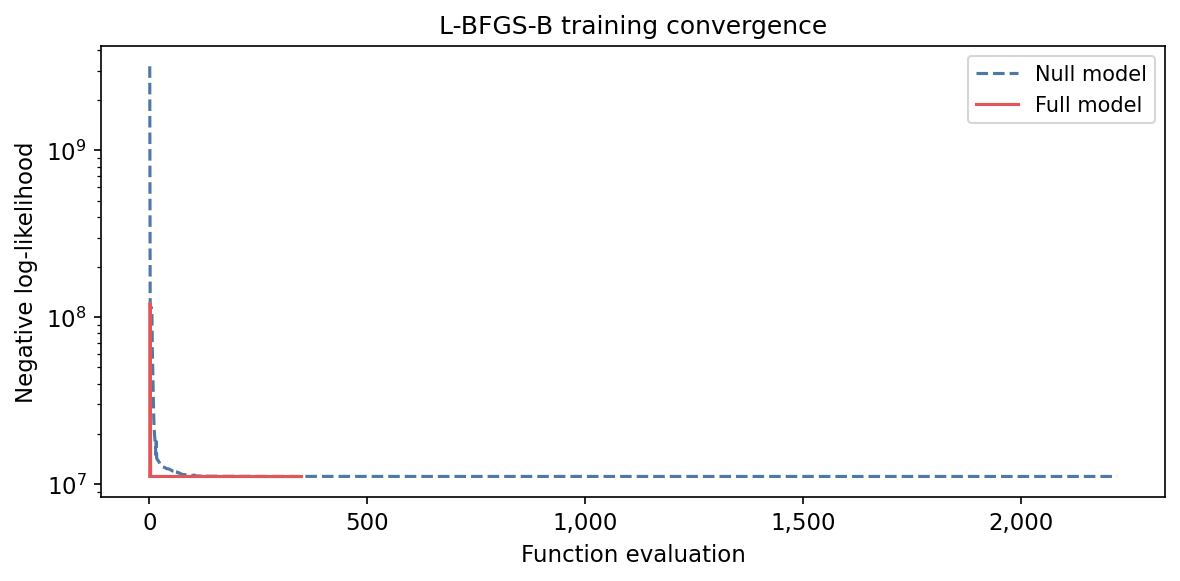
\includegraphics[width=\columnwidth]{fig1_convergence.png}
  \caption{L-BFGS-B training NLL vs.\ function evaluations for the
    null and full models (log scale). Warm-starting the full model
    from the null solution reduces iterations from $\sim$1{,}900 to 300.}
  \label{fig:conv}
\end{figure*}

\subsection{Evaluation Metrics}

We report four metrics on the held-out 2024 test set:
\begin{itemize}
  \item \textbf{NLL}: the optimised training negative log-likelihood.
  \item \textbf{RMSE}: root mean squared error over all nonzero OD cells.
  \item \textbf{Pearson $r$}: linear correlation between predicted $\hat\mu$ and observed $N$.
  \item \textbf{Poisson deviance}: $2\sum_k[N_k\log(N_k/\hat\mu_k) - (N_k-\hat\mu_k)]$, the standard goodness-of-fit measure for count models \cite{Flowerdew1982}.
\end{itemize}

% ─────────────────────────────────────────────────────────────────────────────
\section{Results}

\subsection{Quantitative Comparison}

Table~\ref{tab:metrics} summarises test-set performance.  The full
model improves test Poisson deviance by 0.57\% over the null and
reduces train NLL by 15{,}650, confirming that elevation and weather
carry genuine signal.  RMSE and Pearson $r$ improve only slightly,
reflecting that most OD pairs have low counts ($\approx$1 trip/hour)
and prediction error is dominated by Poisson noise rather than
systematic model error.

\begin{table}[t]
  \caption{Test-set performance, null vs.\ full model.}
  \label{tab:metrics}
  \centering
  \small
  \begin{tabular}{lrrrr}
    \toprule
    Model & NLL (train) & RMSE & $r$ & Pois.\ Dev.\\
    \midrule
    Null  & 11{,}081{,}357 & 1.1520 & 0.0318 & 27{,}879{,}897\\
    Full  & 11{,}065{,}707 & 1.1517 & 0.0324 & 27{,}721{,}769\\
    \bottomrule
  \end{tabular}
\end{table}

\subsection{Fitted Covariate Coefficients}

Table~\ref{tab:coef} lists the fitted $\hat\gamma$ values.
Distance decay is strong: $\exp(\hat\gamma_d\cdot 1) = 0.553$,
meaning demand halves roughly every 1.2 km.
Precipitation is the dominant weather deterrent
($\hat\gamma = -0.521$): a 1 mm/hr rain event reduces expected trips
by $1-e^{-0.521}\approx40\%$.  Temperature has a small positive
effect (+1.2\% per °C), consistent with \citet{Gebhart2014}.
Elevation gain is negligible ($\hat\gamma\approx-10^{-5}$), as
expected given the flat Bay Area topography at dock-to-dock scale.

\begin{table}[t]
  \caption{Fitted covariate coefficients (full model).}
  \label{tab:coef}
  \centering
  \small
  \begin{tabular}{lrr}
    \toprule
    Covariate & $\hat\gamma$ & Marginal effect\\
    \midrule
    Distance (km)        & $-0.592$ & $-45\%$ per km\\
    Holiday              & $-0.233$ & $-21\%$\\
    Elevation gain (m)   & $-0.000011$ & $\approx 0$\\
    Temperature (°C)     & $+0.012$  & $+1.2\%$ per °C\\
    Precipitation (mm/hr)& $-0.521$  & $-40\%$ per mm/hr\\
    Wind speed (m/s)     & $-0.004$  & $-0.4\%$ per m/s\\
    Rel.\ humidity (\%)  & $-0.001$  & $\approx 0$\\
    \bottomrule
  \end{tabular}
\end{table}

\subsection{Temporal Demand Patterns}

Figure~\ref{fig:temporal} shows the fitted temporal fixed effects
$\exp(\eta)$ from the full model.  The hour-of-day profile exhibits
clear commute peaks at 8:00 and 17:00--18:00.  Weekday demand exceeds
weekend demand by approximately 30\%.  Summer months (Jun--Sep) show
$\approx$1.3$\times$ the demand of winter months (Dec--Feb), consistent
with \citet{Gebhart2014}.

\begin{figure*}[t]
  \centering
  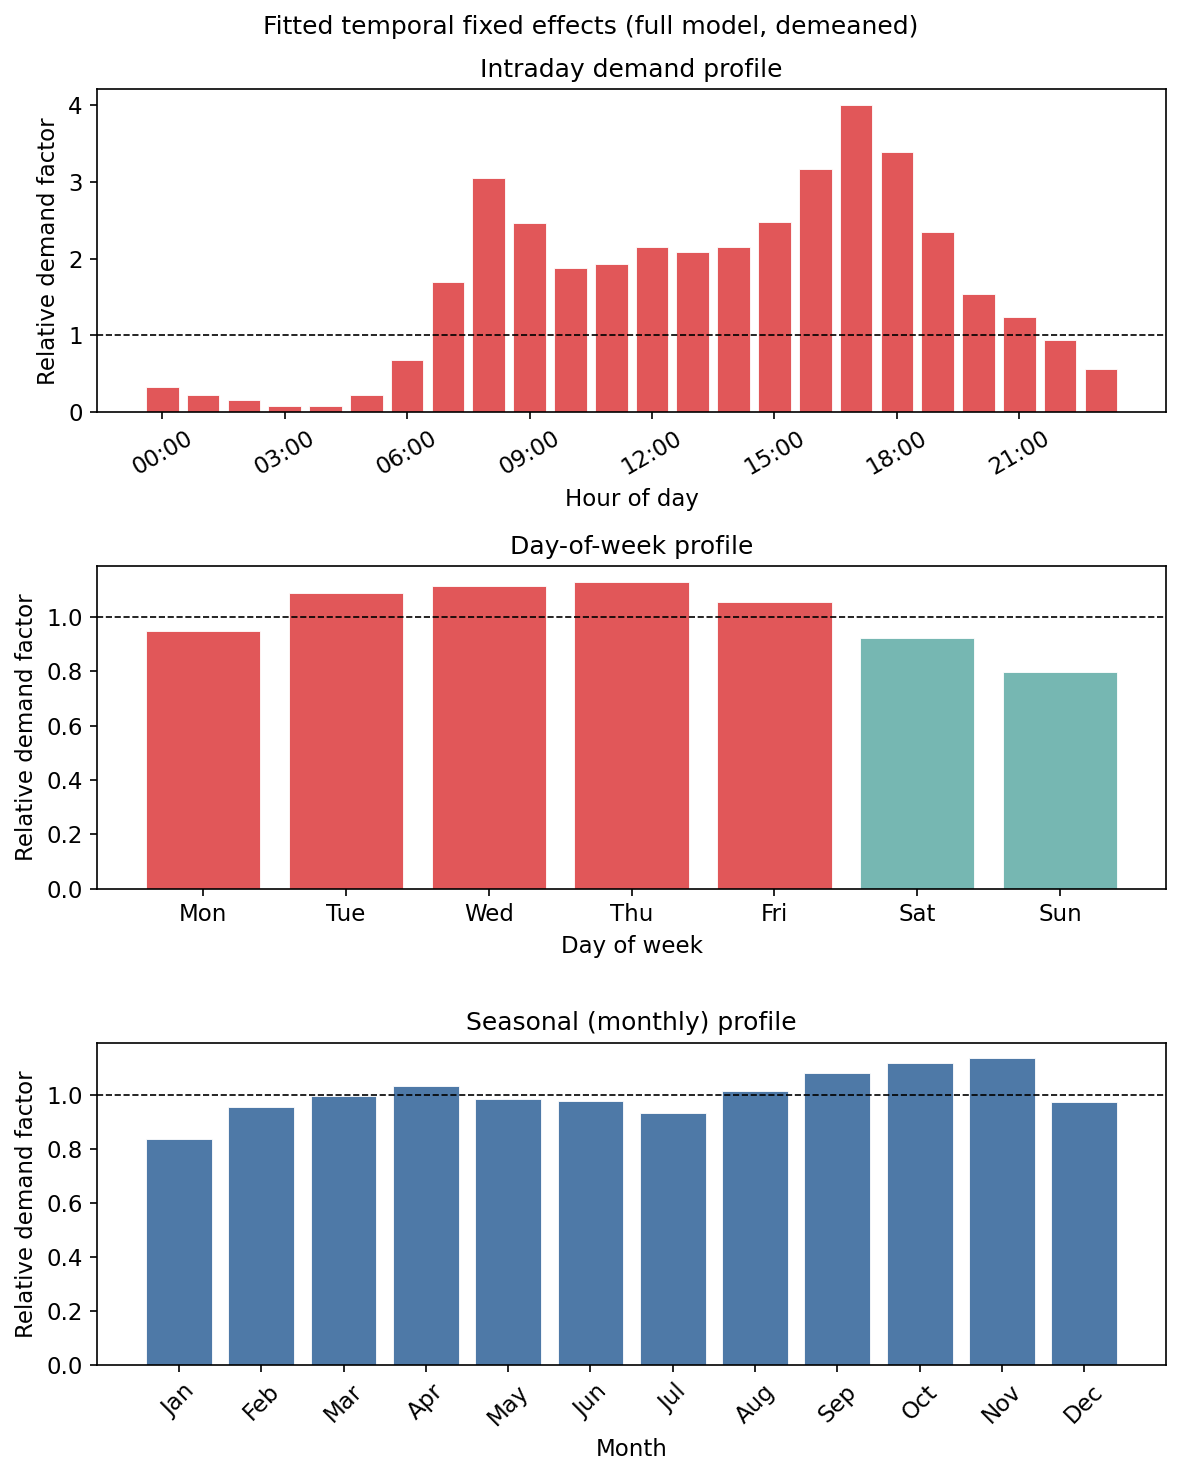
\includegraphics[width=\columnwidth]{fig3_temporal_effects.png}
  \caption{Fitted temporal fixed effects (full model, demeaned).
    Left: intraday demand factor by hour.
    Centre: day-of-week factor (weekdays in red, weekends in teal).
    Right: seasonal (monthly) factor.}
  \label{fig:temporal}
\end{figure*}

\subsection{Distance Decay and Permutation Importance}

Figure~\ref{fig:decay} validates the distance decay by plotting
$\log N_{ij} - \hat\alpha_i - \hat\beta_j$ (observed trips with station
effects removed) against distance for each OD pair.  Under the model
this quantity equals $\hat\gamma_d d + \log S$; the figure confirms the
empirical binned medians closely follow the fitted line, supporting the
log-linear distance specification.

Figure~\ref{fig:import} quantifies feature importance via permutation:
each feature's parameters are zeroed and the increase in NLL is
recorded over three repeats.  Station origin ($\alpha$) and destination
($\beta$) effects dominate, followed by weather as a group
($\Delta\text{NLL}\approx 3{,}500$) and month ($\approx 700$).
Elevation contributes only $\approx 30$ NLL units.

\begin{figure*}[t]
  \centering
  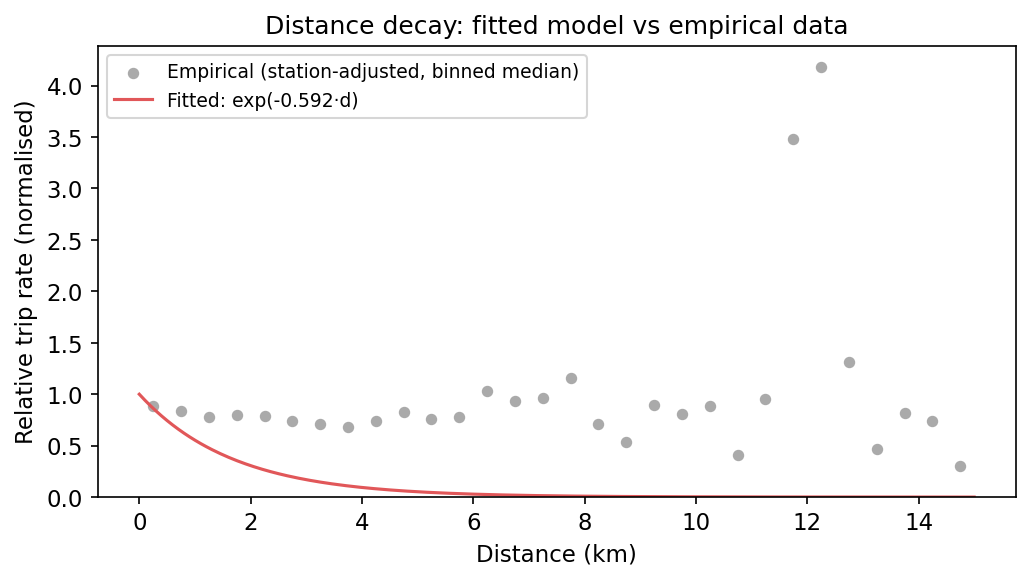
\includegraphics[width=\columnwidth]{fig4_distance_decay.png}
  \caption{Distance decay validation. Each dot is the binned median of
    $\log N_{ij} - \hat\alpha_i - \hat\beta_j$ per OD pair; the red
    line is the model prediction $\hat\gamma_d d + \log S$.
    Empirical medians closely track the fitted line.}
  \label{fig:decay}
\end{figure*}

\begin{figure*}[t]
  \centering
  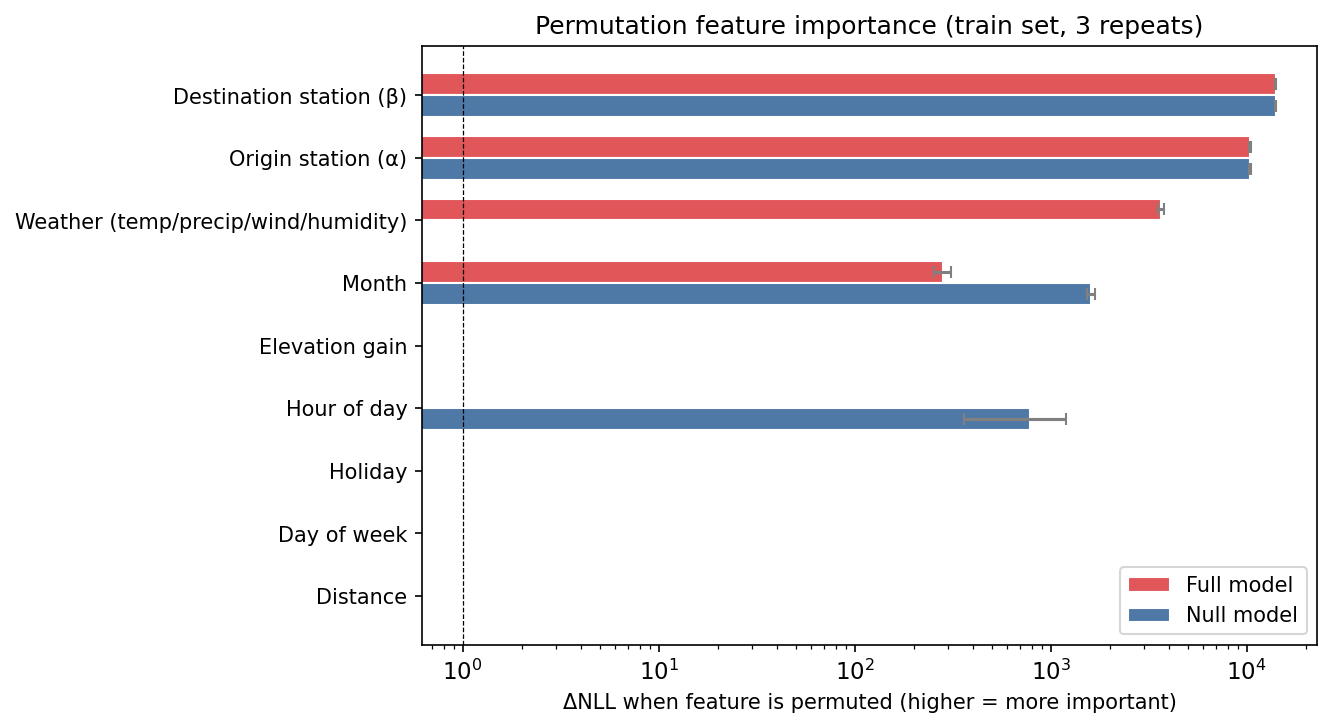
\includegraphics[width=\columnwidth]{fig5_importance.png}
  \caption{Permutation feature importance ($\Delta$NLL, 3 repeats).
    Station fixed effects dominate; weather contributes meaningfully;
    elevation is marginal.}
  \label{fig:import}
\end{figure*}

% ─────────────────────────────────────────────────────────────────────────────
\section{Discussion}

\textbf{Model fitness.}
The Pearson $r\approx 0.032$ appears low but is typical for
highly sparse count matrices where the majority of cells have $N=1$
and Poisson noise is irreducible.  The Poisson deviance is the
more meaningful metric; the 0.57\% improvement of the full model
represents a reduction of 158{,}128 deviance units.

\textbf{Elevation.}
We expected a negative elevation coefficient (climbs discourage
cycling), and indeed $\hat\gamma_{\rm elev}<0$, but the magnitude is
negligible because the majority of Bay Area dock-to-dock elevation
differences are $<20$ m.  A similar model applied to a hilly system
(e.g.\ San Francisco's pre-dockless network) might show a stronger
signal.

\textbf{Ridge on $\boldsymbol\gamma$ only.}
Penalising only the continuous covariates and not the station or
temporal fixed effects is a deliberate modelling choice: the FEs are
identified by the marginal count totals (a sufficient statistic under
Poisson), whereas the covariates share scale information and benefit
from mild shrinkage.

\textbf{Limitations.}
Area-wide weather averages ignore spatial heterogeneity within the
Bay Area (e.g.\ fog in the Sunset district vs. sun in Fremont).
Per-station weather would break the M$\cdot$S factorisation and require
either sparse approximations or a slower $O(I^2 T)$ solver.
A negative-binomial extension could absorb overdispersion not captured
by the fixed effects.

% ─────────────────────────────────────────────────────────────────────────────
\section{Conclusion}

We presented a Poisson gravity model for hourly bike-share OD demand
that combines station fixed effects, temporal fixed effects, and
continuous covariates (distance, elevation, weather) with an efficient
$O(I^2)+O(T)$ gradient factorisation.  Fitted on 4.7M Bay Wheels trips,
the model recovers expected covariate signs: strong distance decay
($-45\%$ per km), holiday suppression ($-21\%$), and precipitation as
the dominant weather deterrent ($-40\%$ per mm/hr).  Elevation is
negligible at Bay Area scale.  The full model improves out-of-sample
Poisson deviance by 0.57\% over the distance-only null, confirming
that area-wide weather adds genuine predictive signal.  Code and
pretrained model bundles are available at
\url{https://github.com/rcatullo/baywheels-od-demand}.

% ─────────────────────────────────────────────────────────────────────────────
\printbibliography

\end{document}
